% Created 2018-01-09 mar 00:45
% Intended LaTeX compiler: pdflatex
\documentclass[xcolor={usenames,svgnames,dvipsnames}]{beamer}
\usepackage[utf8]{inputenc}
\usepackage[T1]{fontenc}
\usepackage{graphicx}
\usepackage{grffile}
\usepackage{longtable}
\usepackage{wrapfig}
\usepackage{rotating}
\usepackage[normalem]{ulem}
\usepackage{amsmath}
\usepackage{textcomp}
\usepackage{amssymb}
\usepackage{capt-of}
\usepackage{hyperref}
\usepackage{color}
\usepackage{listings}
\usepackage{mathpazo}
\usepackage{gensymb}
\usepackage{amsmath}
\bibliographystyle{plain}
\AtBeginSubsection[]{\begin{frame}[plain]\tableofcontents[currentsubsection,sectionstyle=show/shaded,subsectionstyle=show/shaded/hide]\end{frame}}
\AtBeginSection[]{\begin{frame}[plain]\tableofcontents[currentsection,hideallsubsections]\end{frame}}
\usepackage[emulate=units]{siunitx}
\sisetup{fraction=nice, decimalsymbol=comma, retain-unity-mantissa = false}
\newunit{\wattpeak}{Wp}
\newunit{\watthour}{Wh}
\newunit{\amperehour}{Ah}
\hypersetup{colorlinks=true, linkcolor=Blue, urlcolor=Blue}
\renewcommand{\thefootnote}{\fnsymbol{footnote}}
\setbeamercolor{alerted text}{fg=blue!50!black} \setbeamerfont{alerted text}{series=\bfseries}
\usetheme[hideothersubsections]{Goettingen}
\usecolortheme{rose}
\usefonttheme{serif}
\author{Oscar Perpiñán Lamigueiro \\ \url{http://oscarperpinan.github.io}}
\date{}
\title{Tiempo de Retorno Energético de Sistemas Fotovoltaicos}
\hypersetup{
 pdfauthor={Oscar Perpiñán Lamigueiro \\ \url{http://oscarperpinan.github.io}},
 pdftitle={Tiempo de Retorno Energético de Sistemas Fotovoltaicos},
 pdfkeywords={},
 pdfsubject={},
 pdfcreator={Emacs 25.2.2 (Org mode 9.1.4)}, 
 pdflang={Spanish}}
\begin{document}

\maketitle

\begin{frame}[label={sec:org464a5c3}]{Introducción}
A lo largo de su ciclo de vida, además de producir energía y diferentes
residuos, un sistema generador requerirá el empleo de energía para:

\begin{itemize}
\item Fabricación de componentes

\item Tratamiento del terreno

\item Transporte e instalación de los equipos

\item Combustible necesario para su funcionamiento

\item Reposición de equipos que agotan su ciclo

\item \ldots{}
\end{itemize}
\end{frame}

\begin{frame}[label={sec:org4ba609d}]{Ciclo de Vida}
\begin{center}
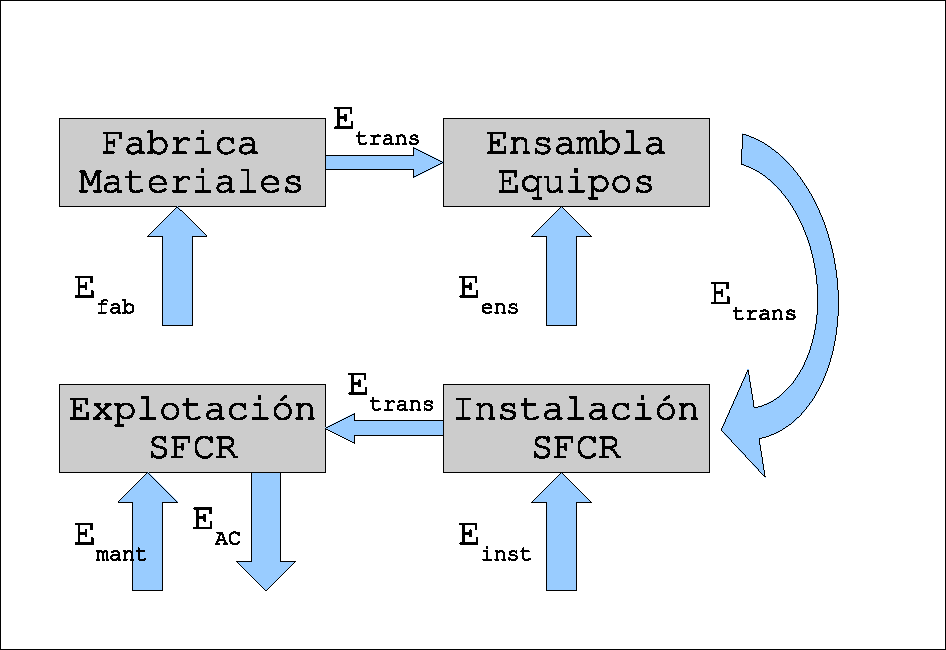
\includegraphics[width=.9\linewidth]{../figs/LCAFlujo.pdf}
\end{center}
\end{frame}

\begin{frame}[label={sec:org4f7efe8}]{Fuentes de Información}
\begin{itemize}
\item \alert{Inventarios de Ciclos de Vida} (\emph{Life Cycle Inventory,} LCI) de los
procesos empleados para implementar un SFCR. A partir de estos LCIs
es posible estimar el impacto energético asociado.

\begin{itemize}
\item Incertidumbre alta en módulos FV (40\%)
\end{itemize}

\item \alert{Radiación global} del lugar en el que el SFCR va a desempeñar sus
funciones

\item \alert{Características técnicas de los diferentes componentes} del SFCR que
permitan estimar la energía producida a lo largo de toda su vida
útil.
\end{itemize}
\end{frame}

\begin{frame}[label={sec:orgb9e08cf}]{Energy PayBack Time}
\begin{columns}
\begin{column}{0.8\columnwidth}
\begin{center}
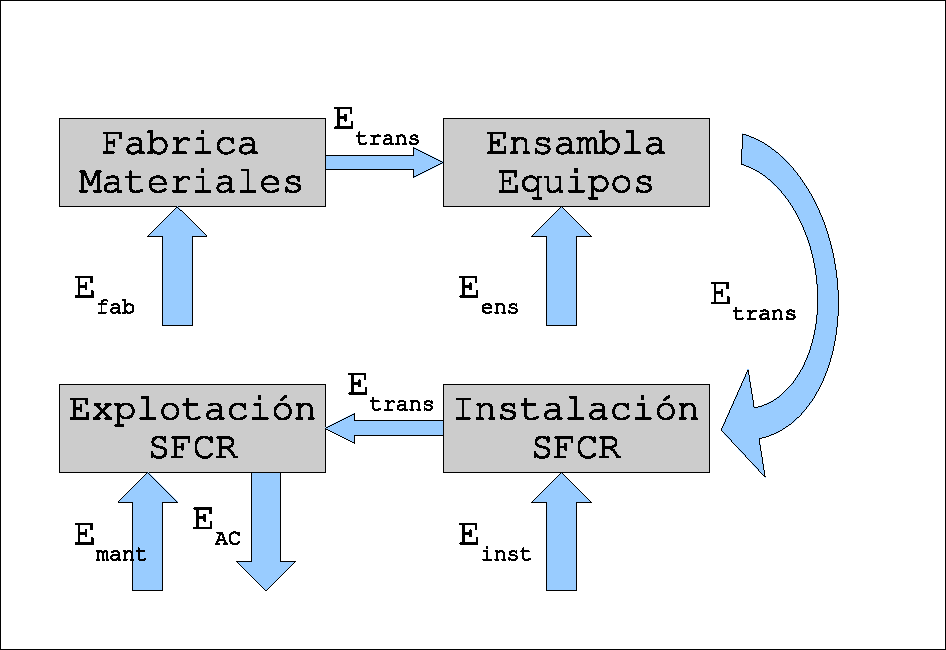
\includegraphics[width=.9\linewidth]{../figs/LCAFlujo.pdf}
\end{center}
\end{column}

\begin{column}{0.25\columnwidth}
\[
  EPBT=\frac{E_{LCA}}{E_{ac}}
\]
\end{column}
\end{columns}
\end{frame}


\begin{frame}[label={sec:org61dcb38}]{La cuestión del mix energético}
\begin{itemize}
\item \alert{La energía primaria depende de la eficiencia de conversión del
sistema energético.}

\begin{itemize}
\item La eficiencia depende de la composición de fuentes energéticas
(mix energético)

\item Eficiencia para zona UCTE: 0.31
\end{itemize}

\item \alert{Proceso productivo de módulo FV es principalmente eléctrico} (80\% de
energía primaria se emplea en electricidad).

\begin{itemize}
\item Centros de fabricación en zonas con alta eficiencia de conversión.

\item Menor impacto ambiental con alta penetración de renovables.
\end{itemize}

\item La \alert{producción de la energía eléctrica} del SFCR se produce
normalmente \alert{lejos del centro de fabricación}

\begin{itemize}
\item Diferente eficiencia de conversión por variación de mix
energético.

\item Menor EPBT inyectando en sistemas poco eficientes.
\end{itemize}
\end{itemize}
\end{frame}

\begin{frame}[label={sec:org677dde0}]{Energía de los principales componentes}
\begin{block}{Seguimiento a Doble Eje}
\begin{center}
\begin{tabular}{lrl}
Componente & (\(MJ_{p}/kWp\)) & (\%)\\
\hline
Módulo & 41819 & 69,54\%\\
Estructura Soporte & 9329 & 15,51\%\\
Mecanismos de seguimiento & 248 & 0,41\%\\
Cimientos (acero) & 3371 & 5,61\%\\
Cimientos (hormigón) & 2445 & 4,07\%\\
Transporte & 1339 & 2,23\%\\
Inversor & 1,091 & 1,81\%\\
Cableado & 497 & 0,83\%\\
Total & 60140 & 100\%\\
\end{tabular}
\end{center}
\end{block}
\end{frame}

\begin{frame}[label={sec:org5379fc7}]{Energía de los principales componentes}
\begin{block}{Seguimiento de Eje Horizontal NS}
\begin{center}
\begin{tabular}{lrl}
Componente & (\(MJ_{p}/kWp\)) & (\%)\\
\hline
Módulo & 41819 & 78,67\%\\
Estructura Soporte & 6108 & 11,49\%\\
Mecanismos de seguimiento & 58 & 0,11\%\\
Cimientos (acero) & 1536 & 2,89\%\\
Cimientos (hormigón) & 1281 & 2,41\%\\
Transporte & 900 & 1,69\%\\
Inversor & 1091 & 2,05\%\\
Cableado & 364 & 0,68\%\\
Total & 53157 & 100\%\\
\end{tabular}
\end{center}
\end{block}
\end{frame}

\begin{frame}[label={sec:orgf878312}]{Energía de los principales componentes}
\begin{block}{Sistemas Estáticos}
\begin{center}
\begin{tabular}{lrl}
Componente & (\(MJ_{p}/kWp\)) & (\%)\\
\hline
Módulo & 41819 & 81,99\%\\
Estructura Soporte & 4459 & 8,74\%\\
Mecanismos de seguimiento & 0 & 0,00\%\\
Cimientos (acero) & 0 & 0,00\%\\
Cimientos (hormigón) & 2352 & 4,61\%\\
Transporte & 1037 & 2,03\%\\
Inversor & 1091 & 2,14\%\\
Cableado & 248 & 0,49\%\\
Total & 51005 & 100\%\\
\end{tabular}
\end{center}
\end{block}
\end{frame}

\begin{frame}[label={sec:orgcc54077}]{Valores de EPBT por sistema}
\begin{center}
\begin{tabular}{lllll}
EPBT & 1st. Quartile & Median & Mean & 3rd Quartile\\
\hline
Doble Eje & 2,4 & 2,6 & 2,7 & 2,82\\
Horizontal-NS & 2,65 & 2,88 & 3 & 3,17\\
Estático & 3 & 3,22 & 3,3 & 3,45\\
\end{tabular}
\end{center}
\end{frame}

\begin{frame}[label={sec:org71816a9}]{Doble Eje}
\begin{center}
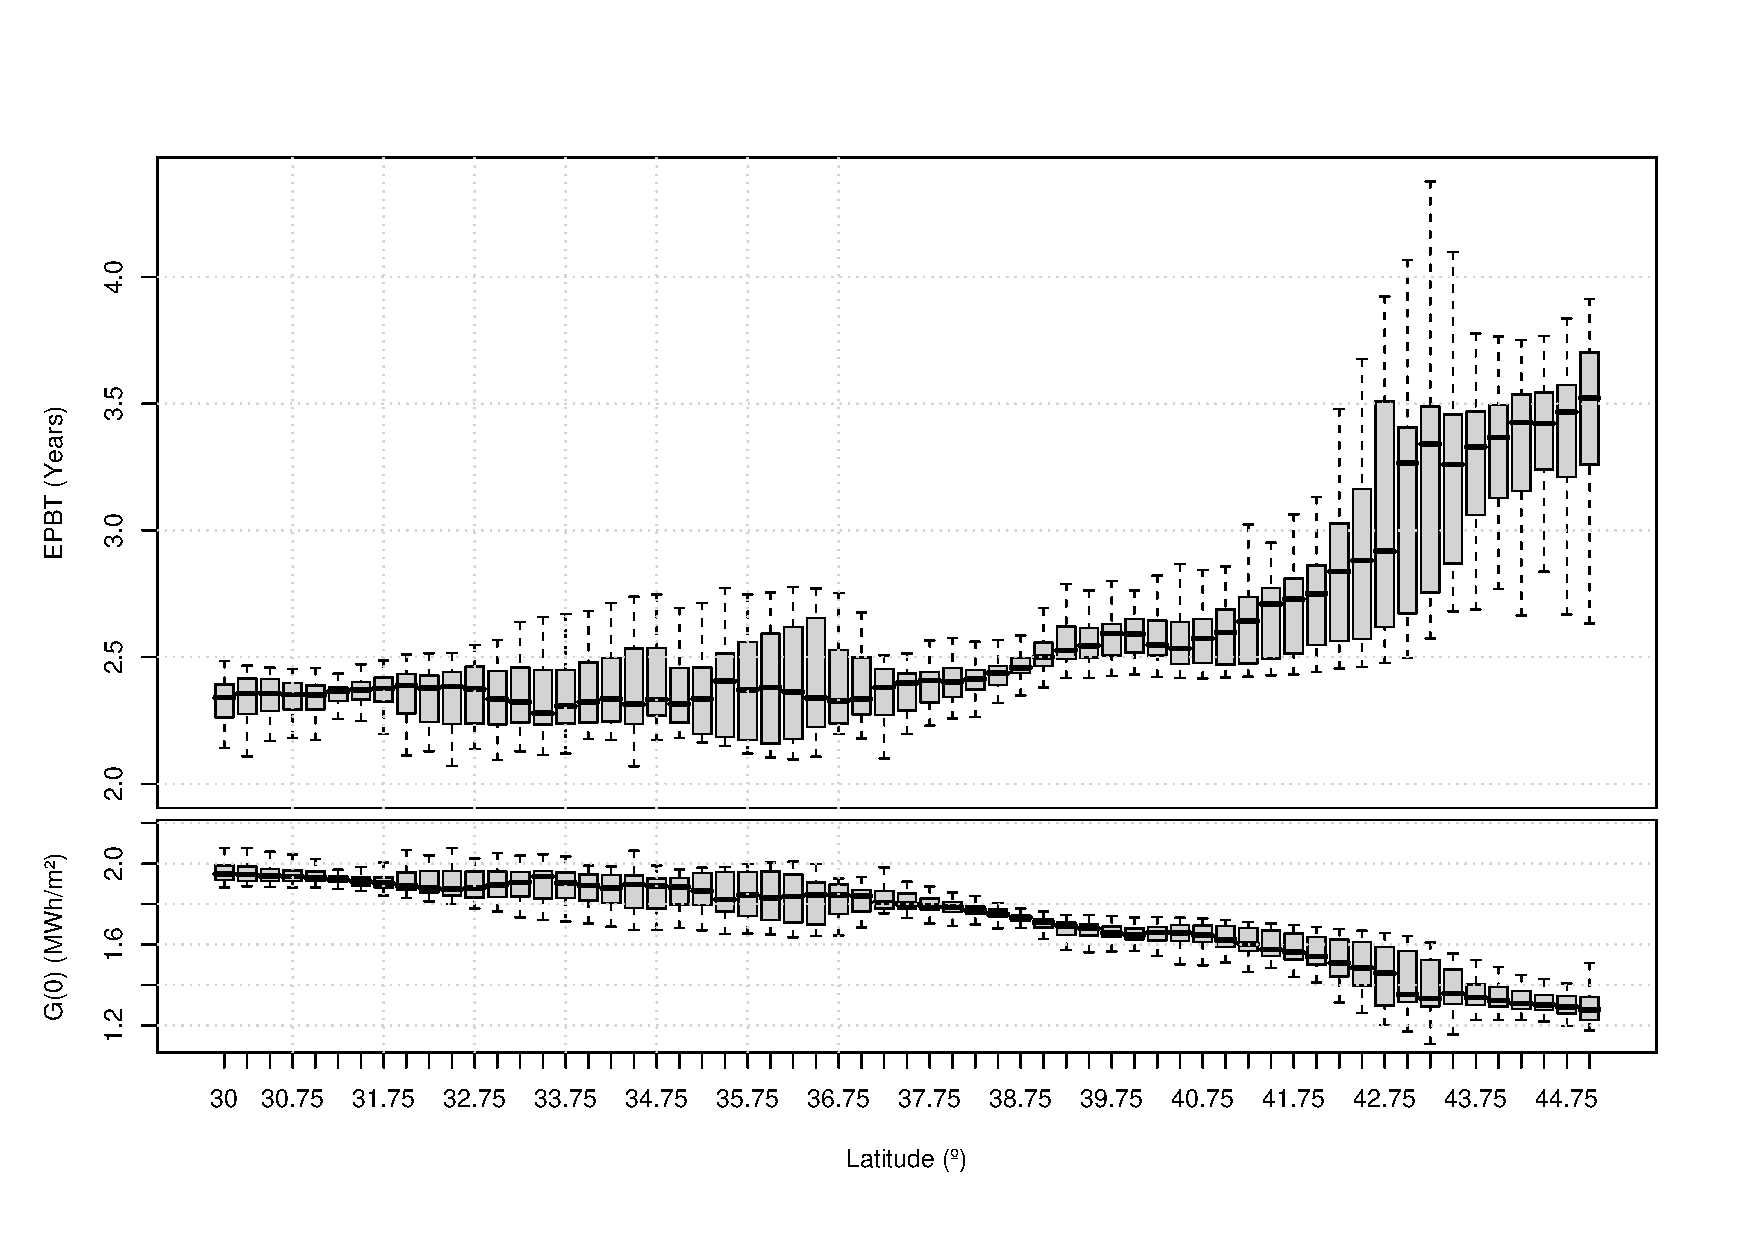
\includegraphics[width=.9\linewidth]{../figs/BoxPlotEPBTEuropa_2x.pdf}
\end{center}
\end{frame}

\begin{frame}[label={sec:org1943512}]{Horizontal NS}
\begin{center}
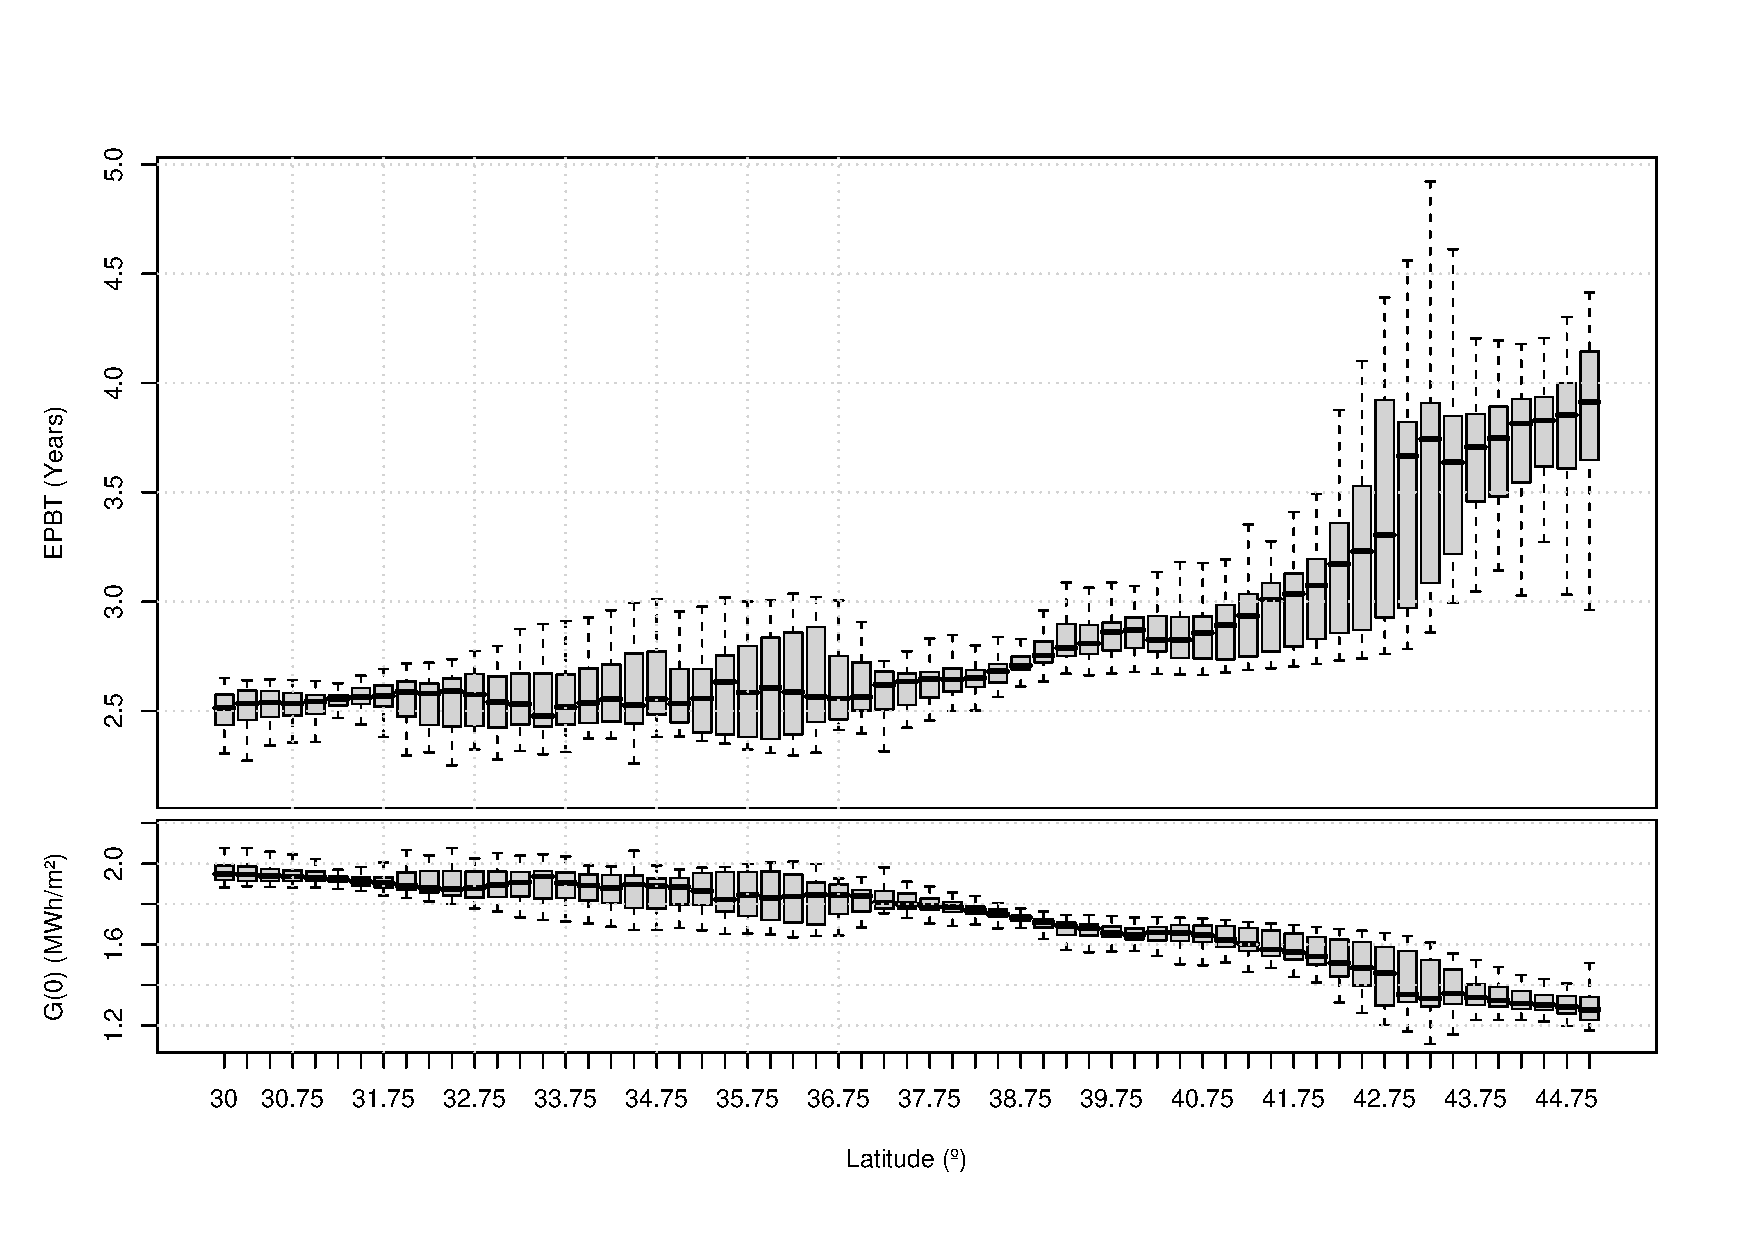
\includegraphics[width=.9\linewidth]{../figs/BoxPlotEPBTEuropa_HorizNS.pdf}
\end{center}
\end{frame}

\begin{frame}[label={sec:orgd6eb6e4}]{Estático}
\begin{center}
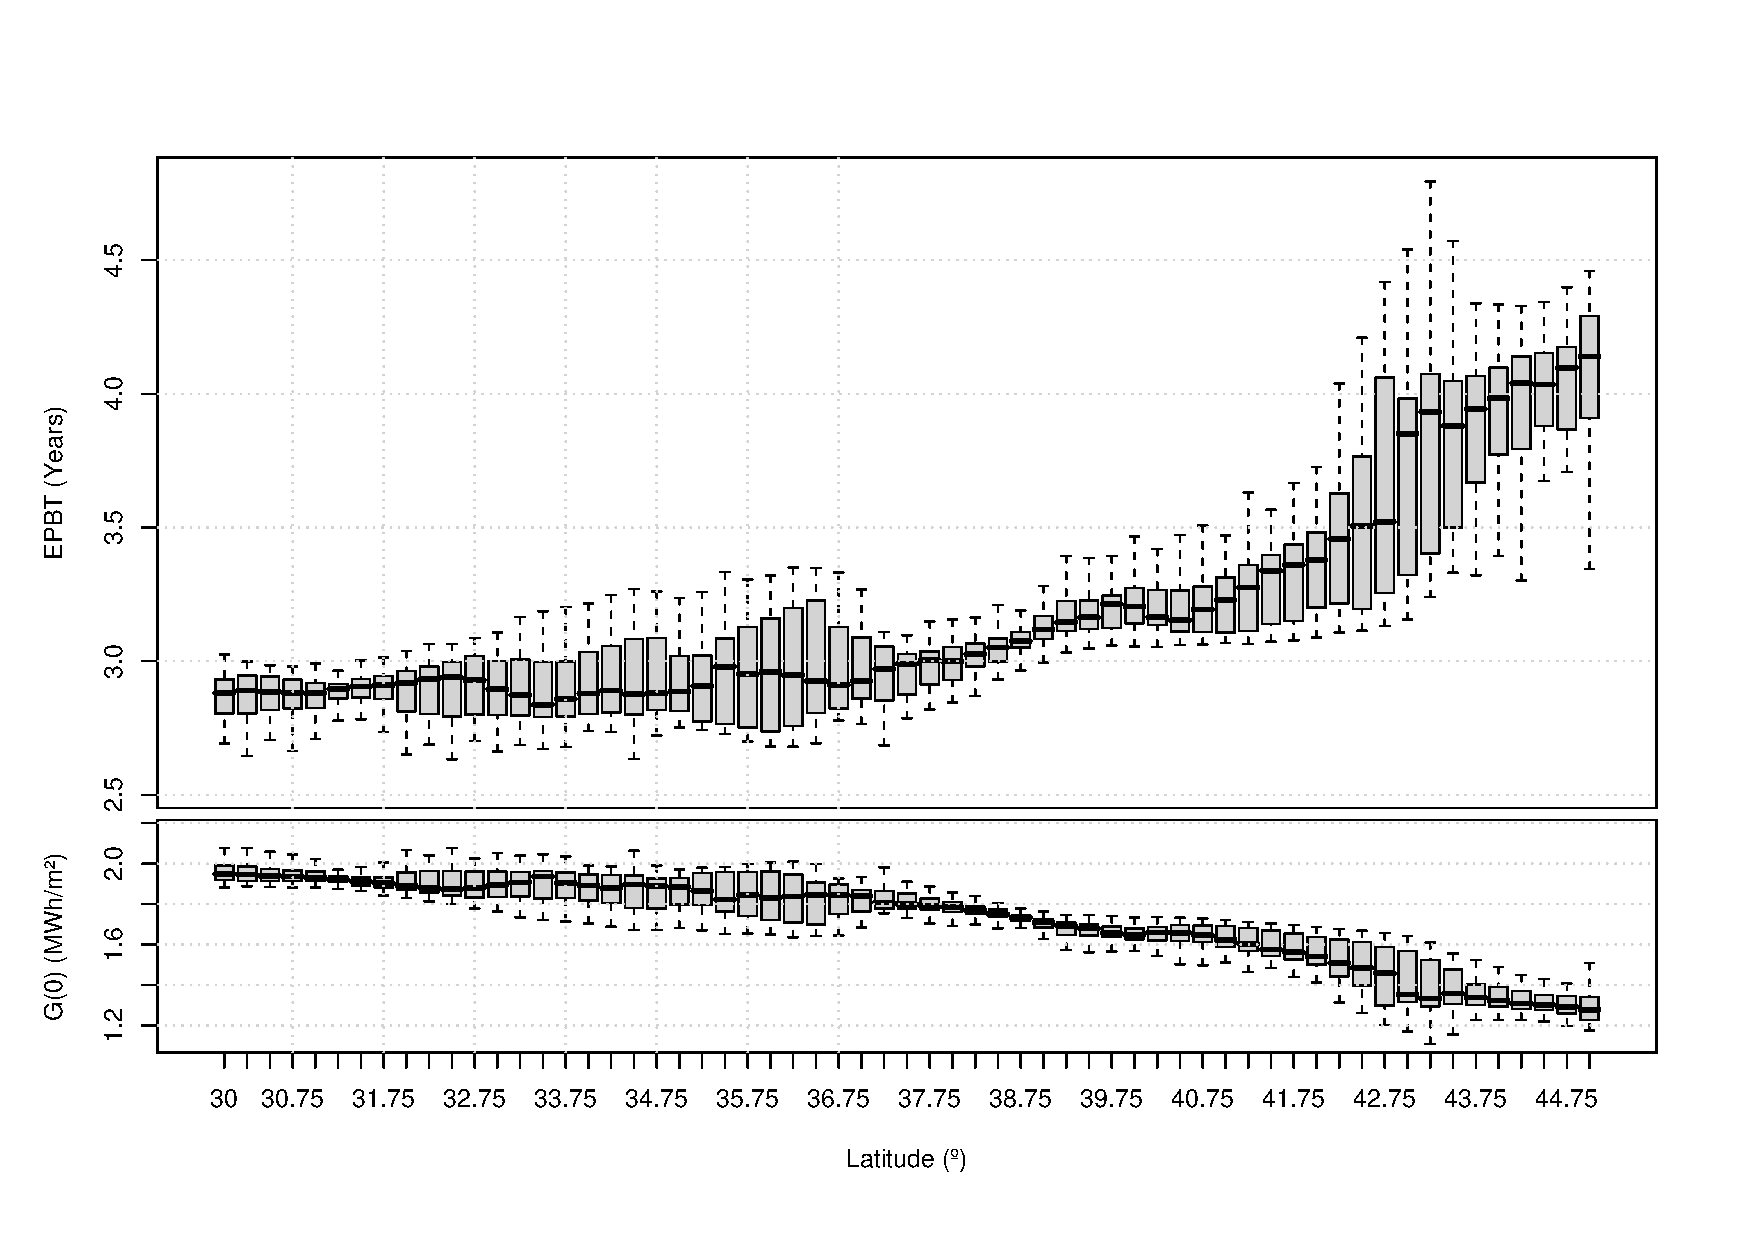
\includegraphics[width=.9\linewidth]{../figs/BoxPlotEPBTEuropa_Fixed.pdf}
\end{center}
\end{frame}

\begin{frame}[label={sec:orgd9bb74d}]{Comparativa}
\begin{center}
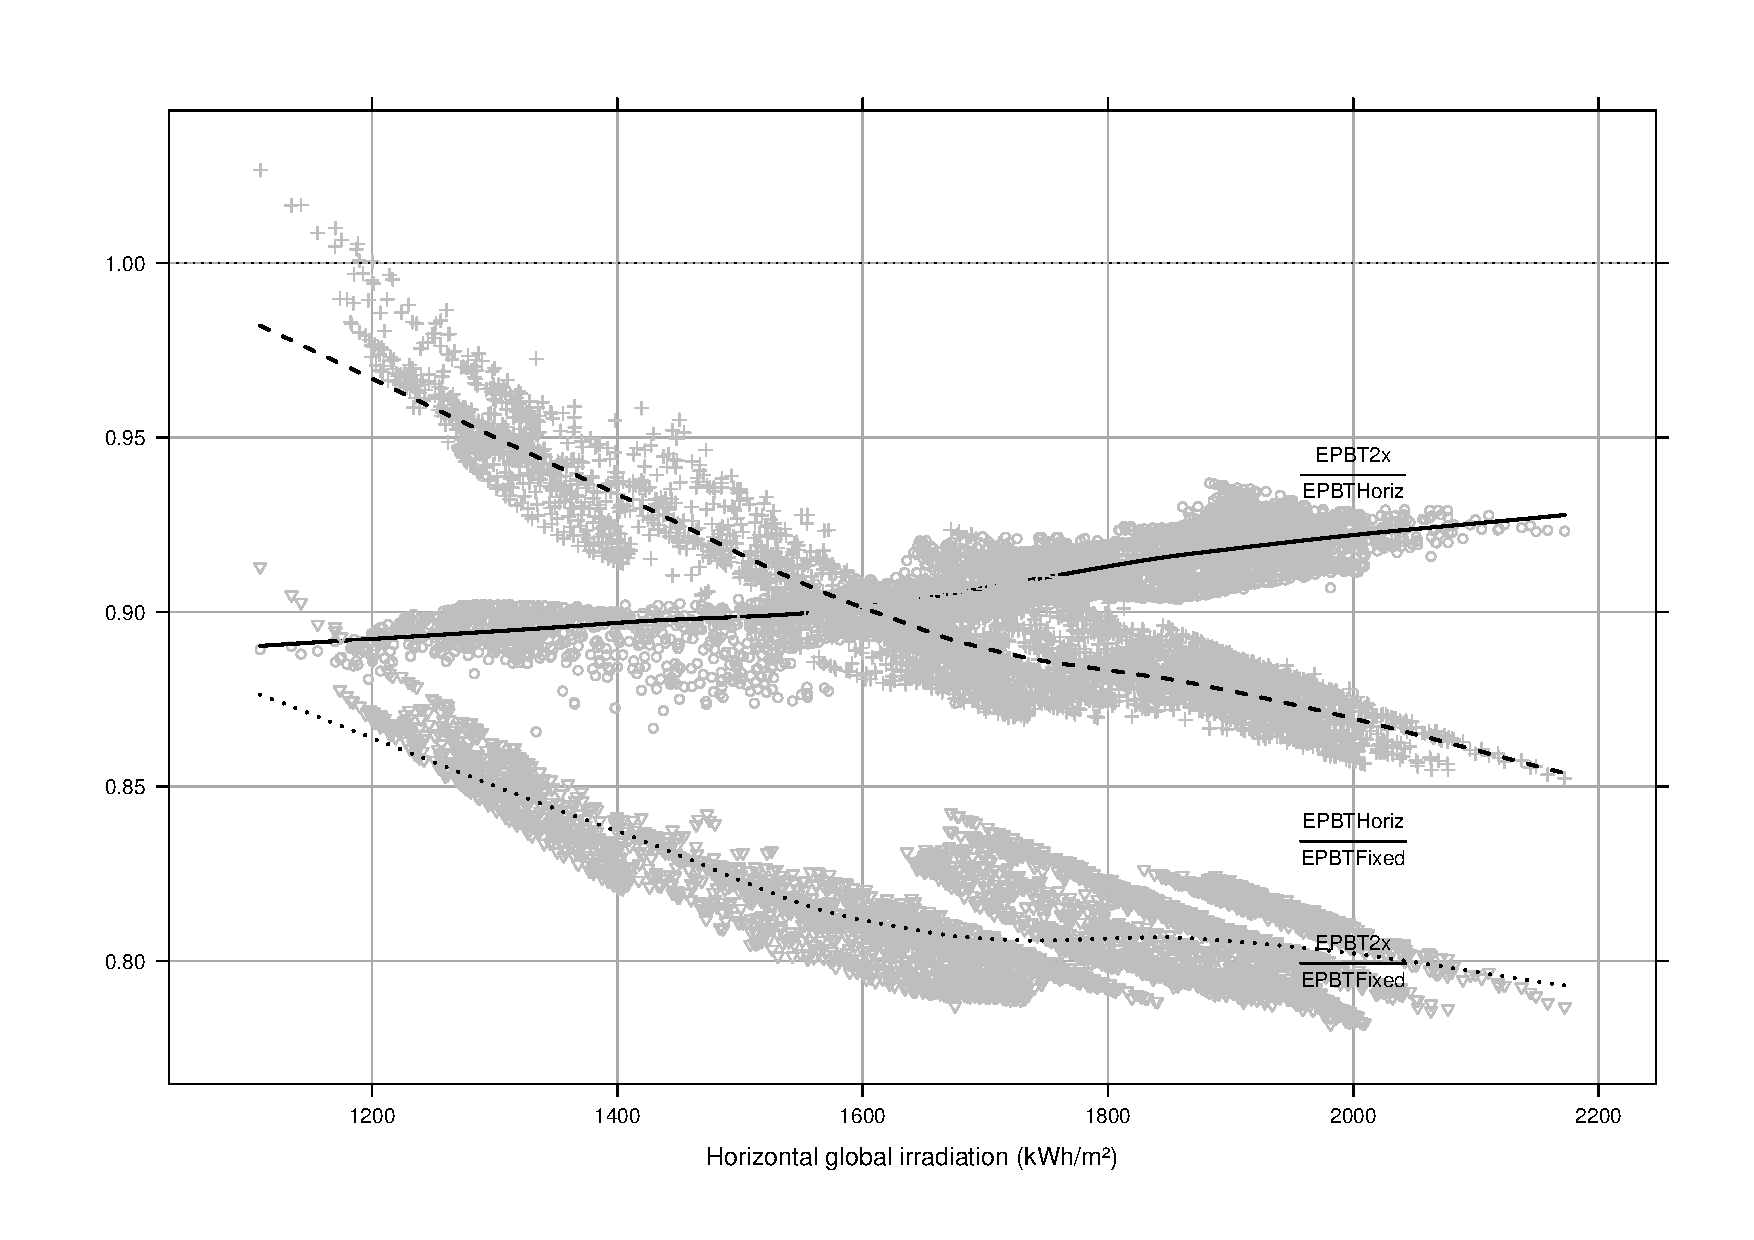
\includegraphics[width=.9\linewidth]{../figs/EPBTEuropavsGh2.pdf}
\end{center}
\end{frame}
\end{document}